% Introducción general del área del conocimiento a la que el tema elegido está vinculado.

% Esta parte es importante para contextualizar el contenido de la obra. Este punto debe de dar evidencias o justificar la esencia o el espíritu del trabajo realizado. Este apartado no es un resumen del trabajo. Es más filosófico y personal que técnico. De alguna manera habla del autor y de lo que pretendía cuando comenzó este trabajo. Esta parte no suele ser muy extensa. Hay que exponer el problema global de manera tan simple como se pueda. Presentar una visión más amplia, más holística del problema. No sobrestimar la familiaridad del lector con el tema del trabajo. No todos los lectores son especialistas en la materia ni la memoria debe de estar redactada para estos. Ayudaría imaginar a una persona, profesor, profesional... que se desenvuelve en un área diferente aunque tenga conocimientos generales técnicos propios de la titulación que se ha cursado. Esta persona es inteligente, tiene su mismo nivel de conocimiento general, pero sabe poco de la literatura, jerga o los trucos que se refieren a su tema particular.

% Escribir de manera que interese vivamente al lector a continuar leyendo. Para los primeros párrafos, la tradición permite la prosa, que es menos dura que el rigor exigido por la escritura científica. Es una buena idea preguntar a alguien que no sea un especialista sobre lo que opina tras leer la memoria. ¿Es una introducción adecuada? ¿Es fácil de seguir? ¿Es interesante?

% Indicar los motivos que han llevado a realizar el TFM y en concreto uno de esta temática. Si había alternativas, hay que valorarlas y justificar las razones de esta decisión. Se debe dejar claro cuál es el tema y porqué es importante.


\chapter{Introducción}
\label{ch:introduccion}

\begin{quote}
  {\bf\textsc{Resumen:}} Este capítulo define los límites del proyecto: problema a resolver, motivos de su elección, objetivos previstos y estructura. Teniendo como propósito convencer al lector y adentrarlo en el área definida como Web Semántica y, darle a conocer la capacidad que esta presenta para integrar información procedente de los Sistemas de Información Geográfica (SIG).
\end{quote}


\section{Introducción}

% Hablar sobre que vamos a estudiar

% Que relevancia tienen los SIG aquí

El trabajo que se presenta a continuación es un estudio sobre la posibilidad de \textbf{integrar Información Geográfica en la Web Semántica mediante el uso de herramientas específicas, a través de la creación de la ontología GEOARES}. A partir de la Información Geográfica disponible en el Instituto de Estadística y Cartografía de Andalucía y centrándonos en la información geoespacial de edificaciones, curvas de nivel y puntos de cotas de Ogíjares (Granada), se realiza una prueba de concepto gracias a las posibilidades de integración que los SIG presentan en la Web Semántica.\\

Actualmente, la gran cantidad de datos presentes en la Web pueden suponer un problema para la búsqueda de información. Este hecho ha ocasionado que organismos tanto privados como públicos hayan optado por la utilización de la Web Semántica. De hecho, la Web Semántica surge como una extensión de la actual Web, para dar solución al problema de que la mayoría de los contenidos de la Web están diseñados para los humanos y no para que los programas de software procesen la semántica de los datos. Para que esto ocurra, es necesario hacer uso de herramientas y tecnologías específicas de la Web Semántica. Dichas tecnologías tratan de aportar información extra a los recursos Web, proporcionando contenidos con significado que permitan mejorar la interoperabilidad entre los Sistemas Informáticos e incluso la aparición de agentes capaces de realizar procesos inteligentes de captura y tratamiento de la información. Por otro lado, los motores de búsqueda clásicos cuando manejan grandes cantidades de datos, en su mayoría no estructurados y generalmente escritos en lenguajes naturales, suelen tener que hacer frente a la imprecisión, es decir, usan similitudes de palabras o estadísticas para encontrar fuentes relevantes, como es el caso de la búsqueda a la que estamos acostumbrados con Google, Yahoo! o Bing.\\

% ejemplo


En la figura \ref{fig:ejemplo-sig} se observa como los motores de búsquedas clásicos (Google) no interpretan la información, sino que simplemente se limitan a devolver resultados a partir de las palabras clave de la búsqueda. En el ejemplo expuesto, se devuelven primero aquellos resultados que contienen en su título la frase ``sistemas de información geográfica''. Esto se realiza así, debido a que la coincidencia de esa frase en el título del documento tiene más relevancia que si lo encontráramos en el contenido textual de dicha página Web.

\begin{figure}[H]
	\centering
	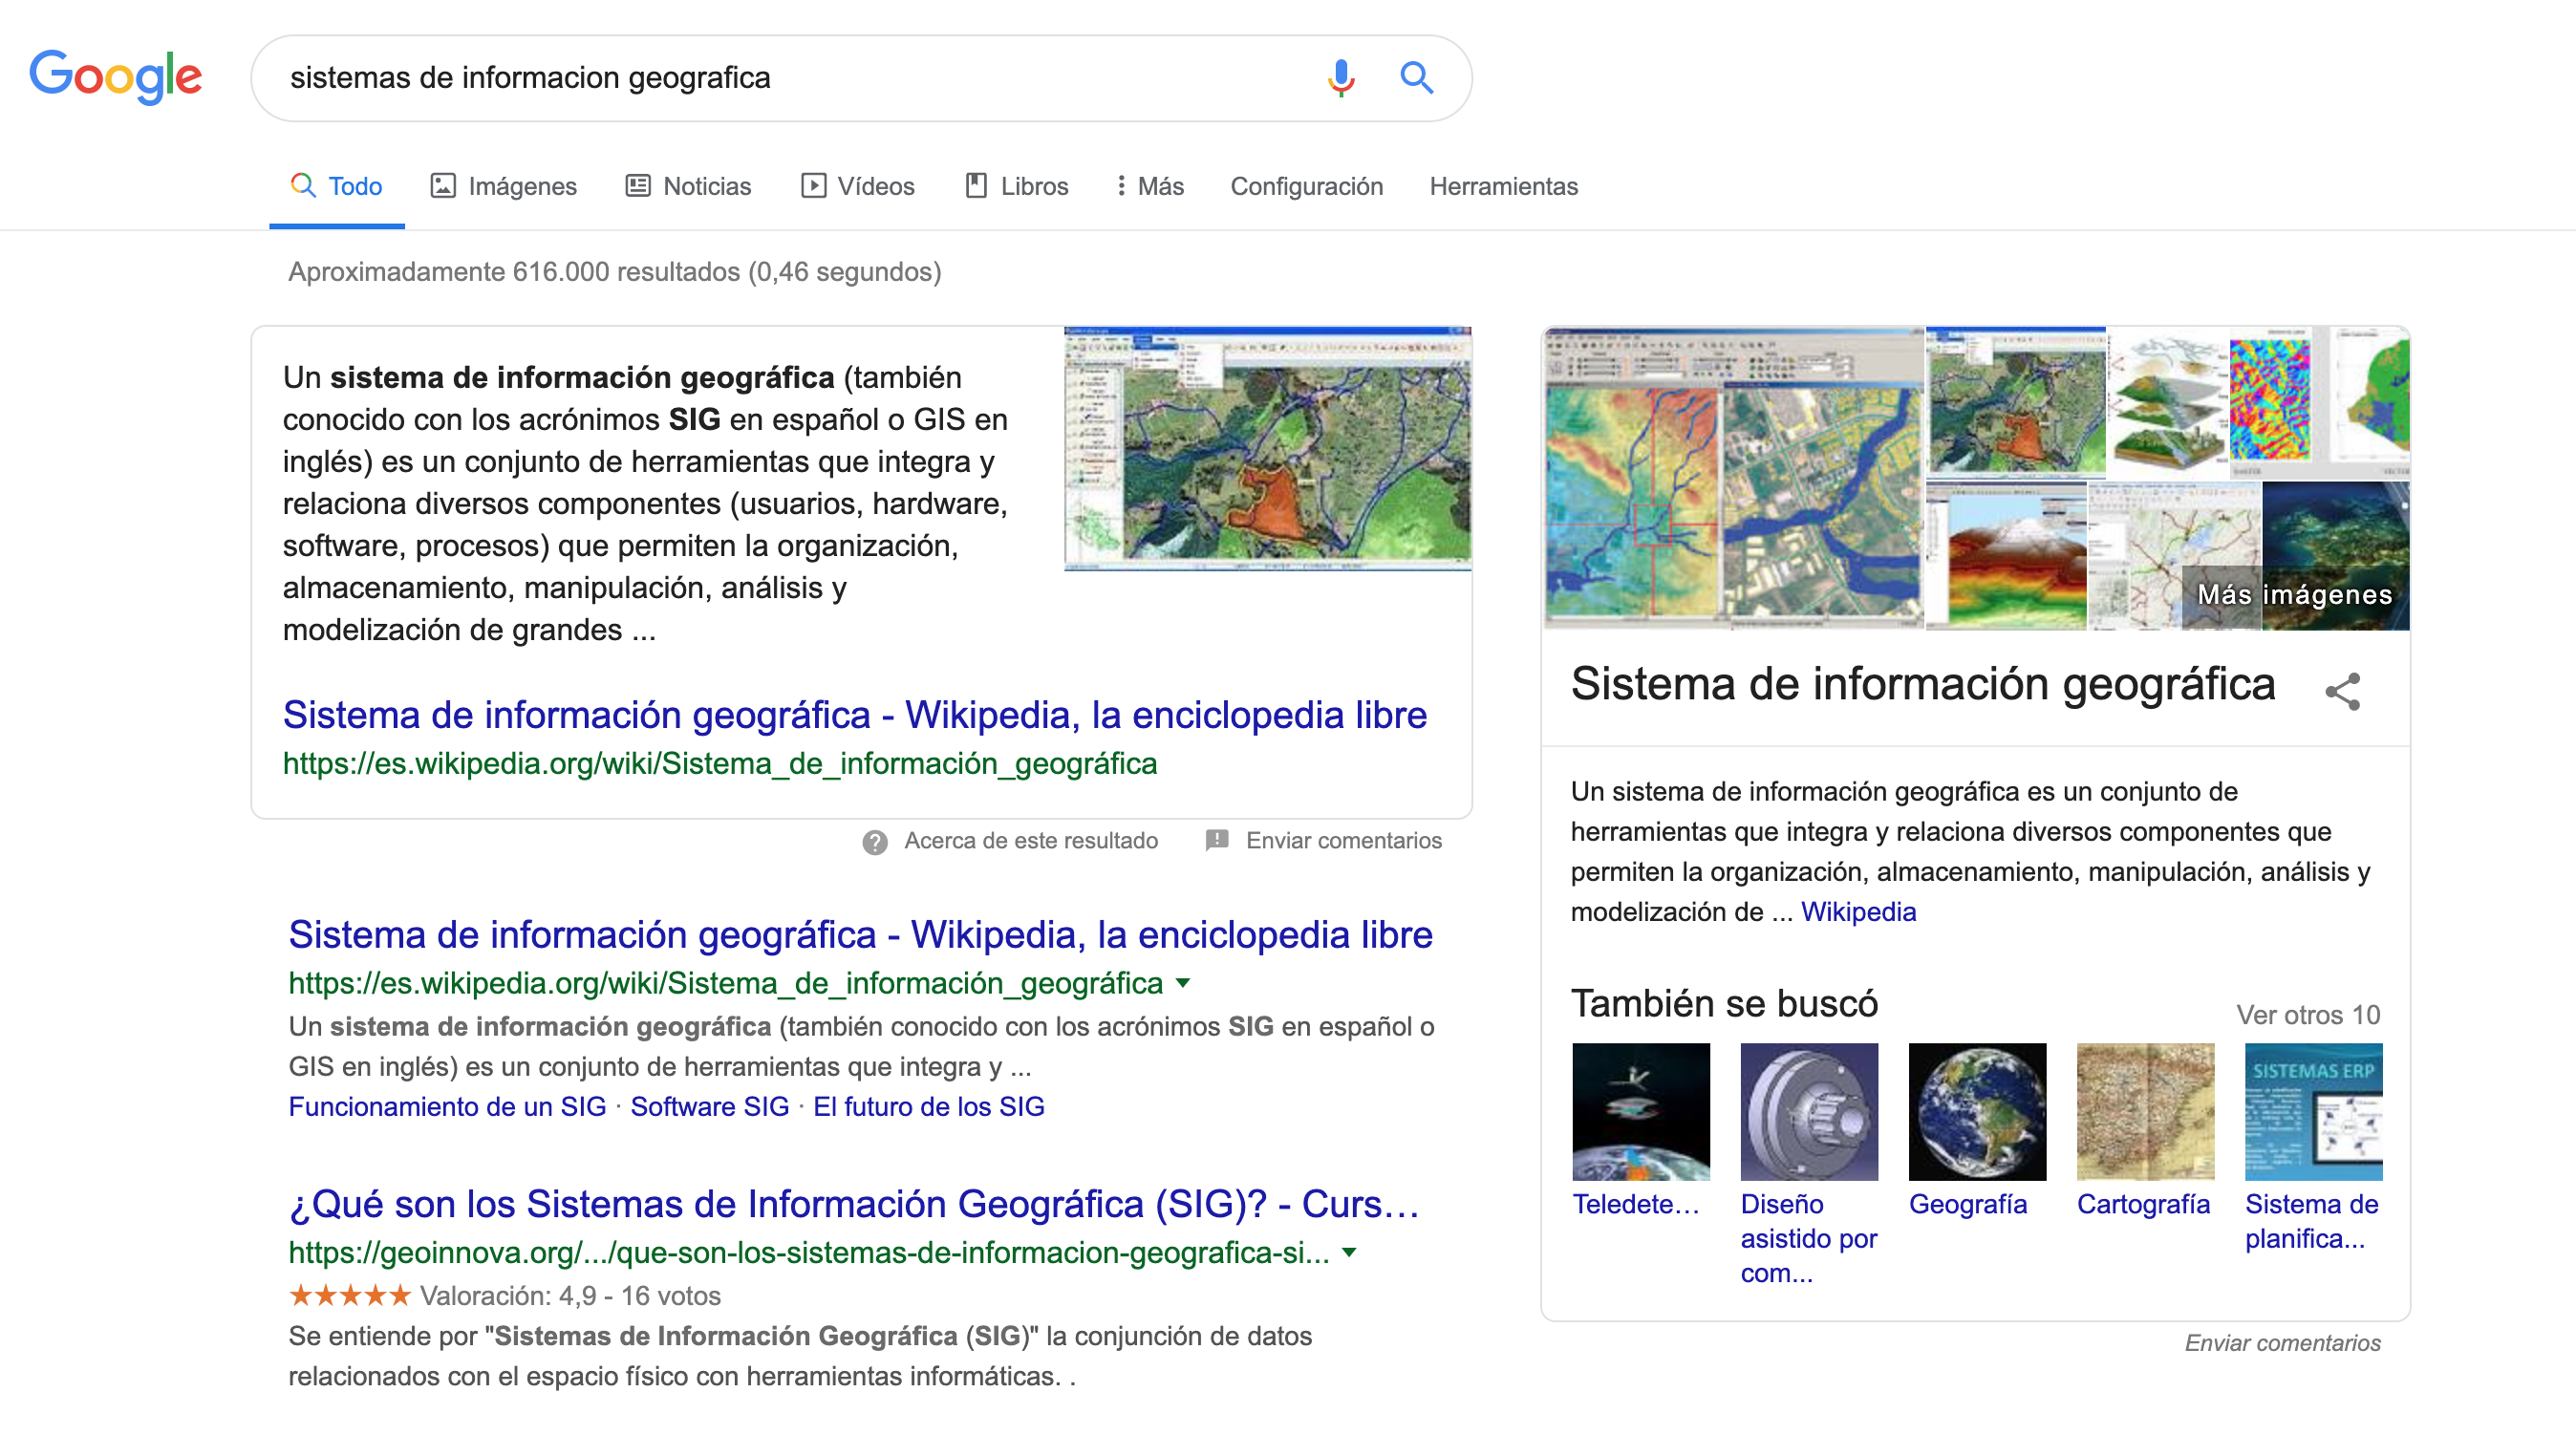
\includegraphics[width=1.07\linewidth]{imagenes/capitulo1/ejemplo-sig1}
	\caption{Ejemplo de búsqueda en Google}
	\label{fig:ejemplo-sig}
\end{figure}

Por contraposición, en el mundo de los SIG, los datos geoespaciales requieren más esfuerzo técnico. Al ser los datos SIG muy relevantes para muchos aspectos de la vida humana, diversos organismos tanto públicos como privados construyen fuentes geoespaciales (mapas) de alta calidad para distintas necesidades: modelos digitales del terreno, mapas de ciudades o mapas meteorológicos, entre otros; además, dictan cómo deben publicarse dichos datos de manera pública. El carácter estructurado de los datos SIG hace posible describirlos con técnicas semánticas, por ejemplo, los objetos espaciales de una capa de un mapa pueden transformarse en instancias de una clase y los atributos pueden convertirse en una propiedad de datos.\\

La capa semántica de los SIG brinda la ventaja de agregar conocimiento de dominio sobre la estructura de los datos (por ejemplo, se puede definir Edificio como una subclase de Sistema Urbano) y de vincular diversos sistemas SIG (por ejemplo, Edificio en un SIG es una subclase de Construcción en otro). Principalmente, por la complejidad de fusionar ambas tecnologías y sus posibilidades, pretendo realizar una prueba de concepto que integre Información Geográfica procedente de la provincia de Granada en la Web Semántica y plasmar dicha información en la creación de una ontología llamada GEOARES.
% es decir, una clase de entidad en un SIG es igual o una subclase de una clase de entidad en otro SIG 


\section{Definición del problema}

% Dedique este tema a aclarar lo que pretende de hecho con su esfuerzo de investigación. El problema es la cuestión a ser respondida por el trabajo, que motivó su realización. Es una cuestión que ya se formó en su mente, derivada de teorías del área investigada y de su observación sobre un fenómeno. Normalmente se utilizan los siguientes subíndenes como medios para determinar claramente los objetivos, lo que también colabora para la delimitación del alcance del trabajo. Está estrechamente vinculado al objetivo general, que normalmente consiste en encontrar la respuesta al problema de investigación.

% ¿Qué has visto que es un problema que necesita solución? ¿Es viable? ¿Puedes hacer? El problema es siempre una dificultad, una laguna.

% Breve descripción antes de poner el objettivo de manera clara y concisa

La Web Semántica permite incorporar información muy diversa, entre ella cabe destacar la Información Geográfica. Con los conocimientos que tengo adquiridos durante el Grado en Ingeniería Informática en el ámbito de los SIG y los de Web Semántica adquiridos durante el Máster Universitario en Ingeniería Informática, pretendo hacer uso de ambas áreas para desarrollar un ejemplo práctico que agregue conocimiento geográfico mediante las herramientas de la Web Semántica. \\ %De tal forma que el trabajo tiene como objetivo la integración de Información Geográfica en la Web Semántica. \\

A partir de los mecanismos para la integración de información procedente de diversas fuentes que ofrece la Web Semántica, se han definido estándares de representación de Información Geográfica mediante herramientas de la Web Semántica. En este proyecto se estudian algunas de las herramientas que se pueden utilizar para representar e integrar Información Geográfica, valorarlas y desarrollar una prueba de concepto. Se trabajará con información geoespacial, concretamente con archivos en formato \textit{Shapefile} de la provincia de Granada, en particular de mi pueblo, Ogíjares, y nos centraremos en la información geoespacial obtenida de edificaciones, puntos de cota y curvas de nivel. En la prueba de concepto, se hará uso de las herramientas destinadas a la generación de información geoespacial propias del área SIG (\texttt{QGIS} para tansformar los \textit{Shapefile}) junto con herramientas de la Web Semántica (\texttt{Protegé}, \texttt{GraphBD}) y otras para representar la información obtenida como resultado (\texttt{R} y \textit{Shiny}). 

%\texttt{QGIS}, para permitir obtener la información de los \textit{Shapefile} a hojas de cálculo; generación de documentos \textit{RDF} con \texttt{Protegé}, para permitir llevar la información de los \textit{Shapefile} hacia documentos en formato \textit{RDF} de manera gráfica; consumo con \texttt{GraphBD},  para permitir la visualización de archivos en formato \textit{RDF} y la realización de las consultas con el lenguaje estándar de consulta geoespacial \textit{GeoSPARQL}; y visualización de la información geoespacial obtenida de las consultas con \texttt{R} para permitir ubicar la información geográfica en un mapa interactivo mediante la librería \textit{Shiny}.


\section{Motivación}

% Uno de los debates más habituales en la utilización de los Sistemas de Información Geográfica en entornos académicos es hasta que punto implican realmente un avance científico, con lo que su presencia como asignatura sería de pleno derecho, o si son sólo una herramienta, poco más que un procesador de textos, que los alumnos deberían aprender por su cuenta y que, como mucho, podría servir para explicar visualmente otros contenidos.

\textit{¿Qué motivación y razones me han llevado a comenzar un proyecto como este?} Cómo Ingeniera Técnica Informática y estudiante del Máster Universitario en Ingeniería Informática, he adquirido a lo largo del Grado y del Máster conocimientos y usos muy diversos que se le puede dar a la tecnología. Después de haber realizado el Trabajo de Fin de Grado en \textit{Análisis de Información Geográfica mediante QGIS y R centrado en el Modelo Digital del Terreno}, he querido seguir cumpliendo el objetivo que me propuse: conocer más el mundo en el que se mueven los SIG, puesto que en estos dos años me es imposible abarcar todas las áreas relacionadas con el mismo. Además de haberme matriculado en el Grado en la asignatura de \textit{Sistemas de Información Geográficos}, destacar que durante la realización del Máster Universitario en Ingeniería Informática, he adquirido algunos conocimientos en la temática de Web Semántica a partir de la asignatura de \textit{Desarrollo de Software basado en Componentes y Servicios} impartida por Manuel Ignacio Capel Tuñón. Es más, las ganas de adentrarme en este mundo, han hecho que durante este año haya asistido al curso de \textit{Web Semántica} del Máster de Desarollo de Software, impartido por diversos profesores, entre ellos el tutor de este TFM. Por esto, con la idea de pasar a un siguiente nivel mi Trabajo de Fin de Grado, surgió este Trabajo de Fin de Máster en el que intento profundizar en la Web Semántica Geoespacial, con el fin de enriquecerme tanto personal como profesionalmente. Con este TFM quiero permitir al lector iniciarse en este tema tan interesante.\\ 

% el profesor (actual tutor) me introdujo en un ámbito que desconocía y del que apenas había oído hablar. 

% hablar sobre los cursos asistidos este año
% hablar sobre la conferencia que fui en Madrid
% hablar sobre la asignatura de SIG en el grado
% hablar sobre la asignatura de Capel

La idea de este proyecto comenzó a tomar forma a principios de curso, tras mantener varias reuniones con el tutor del TFG y ver que posibilidades había de seguir estudiando y ampliando los SIG de manera más práctica y profesional (en el \texttt{Apéndice \ref{ch:ApendiceA}} se encuentra la planificación del TFM). Entonces, partiendo de todos los conocimientos que tengo antes de la realización de este trabajo, me pregunto lo siguiente: \textit{¿existe interoperabilidad\footnote{La interoperabilidad es la capacidad de los Sistemas de Información y de los procedimientos a los que éstos dan soporte, de compartir datos y posibilitar el intercambio de información y conocimiento entre ellos.} en los Sistemas de Información Geográfica?} Este tipo de preguntas ha llevado a cabo el inicio del desarrollo de la prueba de concepto, en donde, gracias a la capa semántica que ofrecen los SIG, es posible integrarlos de manera adecuada en la Web Semántica. En los sucesivos capítulos, iremos detallando cada uno de los conceptos que, a lo largo de esta introducción, se han mencionado.


% coursera
%En este curso verá en que consisten las tecnologías de la Web Semántica y como se utilizan en la web actual. También tendrá la oportunidad de realizar varios proyectos aplicando todas estas tecnologías para resolver los problemas que Marcelo ha comentado anteriormente. Por ejemplo, ¿le gustaría que Google entendiera cada uno de los componentes de su página web? O si usted tienen una tienda virtual, ¿le gustaría que Google fuera capaz de identificar los distintos productos que forman parte de su tienda virtual y los desplegara al momento de hacer una búsqueda? Esto se consigue usando [DESCONOCIDO] y les mostraremos como se relaciona en este curso con las tecnologías de la Web Semántica.

%Además, ¿le gustaría poder acceder a la Wikipedia como si fuera una tabla Excel? ¿O le gustaría poder conocer como han hecho los gobiernos para hacer públicos sus datos y de esta manera permitir que los ciudadanos puedan acceder a la información de como se gastan sus impuestos, o puedan entender de una manera más sencilla como le afecta una ley? ¿O le gustaría saber como hacen los biólogos para compartir sus datos en la web?


\section{Premisas e hipótesis}

% La mejor forma de determinar el tema abordado es a través de premisas e hipótesis. La hipótesis consiste en una afirmación que usted considera verdadera y que va a probar o buscar probar a lo largo de su trabajo. Otra forma es delimitar el problema en forma de una pregunta de partida. Las hipótesis presentadas aquí son probadas en su trabajo es lo que llamas de tesis.

La realización de este trabajo ha partido de varios supuestos básicos: el primero parte de la posibilidad de la interoperabilidad que presentan los datos con Información Geográfica. Asumiendo, que los datos geoespaciales interoperables pueden ser utilizados por diferentes programas y aplicaciones permitiendo así el intercambio de información y conocimiento entre ellos. El segundo supuesto es un hecho y es la utilidad de integrar información estructurada de diversas fuentes en la Web Semántica gracias a la estructura que estos presentan mediante su representación en una ontología para así permitir que la información contenida en las páginas Web sea entendible tanto por humanos como por máquinas. Y por último, considero que este tema puede resultar de interés en el ámbito tecnológico en general, y de los Ingenieros en Informática en particular.


\section{Objetivos}

% Es la respuesta al problema especificado anteriormente, es decir, lo que se pretende hacer y que, después de alcanzado, habrá terminado el trabajo. Algunos verbos utilizados para determinar el objetivo general: contribuir / facilitar / subsidiar / proponer / aclarar / permitir / agregar / comprender.

Este apartado recoge los objetivos iniciales marcados para la realización del TFM, especificando los propósitos que se esperan conseguir del mismo. A continuación, se detallan tanto los objetivos generales como específicos.

\subsection{Objetivo general}

El objetivo de este proyecto es profundizar \textbf{en las herramientas de la Web Semántica que se pueden utilizar para representar e integrar Información Geográfica, valorarlas y desarrollar una prueba de concepto con la creación de la ontología GEOARES}. Para ello, se hará uso de las distintas posibilidades que existen actualmente en la Web Semántica Geospacial. Así que, mediante este trabajo se adquirirá experiencia en la Web Semántica y en el uso de sus herramientas para combinar información procedente de los SIG.

\subsection{Objetivos específicos}
\label{ch:objetivos}

% Los objetivos específicos detallan los objetivos generales a través de etapas o fases de investigación. Se deben utilizar verbos en el infinitivo, señalando las acciones propuestas para alcanzar el objetivo general. Los verbos utilizados aquí son los de acción, que serán utilizados en la metodología.

% Comprobar si los objetivos puestos del principio corresponden con los objetivos que he cumplido al terminar el trabajo

En el subapartado anterior, se mencionan a grandes rasgos los objetivos que vamos a lograr con dicho estudio y aplicación. A continuación, se detallan los objetivos más específicos del proyecto:

\begin{enumerate}
	
	\item \textbf{Comprender la relación existente entre los Sistemas de Información Geográfica y la Web Semántica}, a priori dos áreas completamente diferentes.
	
	\item \textbf{Hacer uso de fuentes de información geoespacial}, con las que obtener datos públicos geográficos de buena calidad.
	
	\item \textbf{Localizar diversas herramientas de la Web Semántica} que se puedan utilizar para representar e integrar Información Geográfica.
	
	\item Aprender a \textbf{agregar conocimiento de dominio geoespacial sobre la estructura de los datos} mediante el empleo de herramientas de la Web Semántica como Protegé.
		
	\item \textbf{Aprender a crear ontologías y poblarlas}  mediante información geográfica existente.
	
	\item Apreciar las carencias o mejoras que supone usar \textbf{Protegé frente a otro tipo de herramientas}.
	
	\item Conocer cuál es la \textbf{estructura de los datos geoespaciales y sus especificaciones para la realización de las consultas con el lenguaje GeoSPARQL}.
	
	\item Aprender a \textbf{ubicar información geoespacial en un mapa mediante el uso de la biblioteca Leaflet}.
	
	\item Mostrar algunos \textbf{métodos de trabajo}, estrechamente adaptados al tratamiento de Información Geográfica en la Web Semántica.
	
	\item \textbf{Aportaciones a la comunidad o al lector}, para que el proyecto sirva como puerta de acceso al mundo de la Web Semántica y, en particular, al de la Web Semántica Geoespacial, y facilite el acceso a parte de los conocimientos actuales disponibles.
	
	\item \textbf{Aportaciones hacia mi persona} en la puesta en práctica y adquisición de conocimiento de los anteriores puntos.
	%\item \textbf{Aportaciones hacia mi persona} en la adquisición de conocimientos de la Web Semántica, creación de ontologías, manejo de herramientas semánticas como Protegé y aprendizaje para la creación de un mapa interactivo mediante la librería Shiny de R.	

	
	%\item \textbf{Análisis exhaustivo de los MDT}, contemplando las posibilidades que presentan para su futura aplicación en el ámbito de los SIG.
	
	%\item Aprender a \textbf{manipular información del terreno} mediante el empleo de herramientas como QGIS y R.
	
	%\item Apreciar las carencias o mejoras que supone el \textbf{uso de R frente a QGIS}.
	
	%\item Analizar un MDT con diversos paquetes de R y en consecuencia, \textbf{crear un paquete en R} que encapsule el análisis de sombras.
	
	%\item \textbf{Conocer diversas fuentes de información}, con las que obtener datos precisos del terreno y de buena calidad.
	
	%\item Mostrar algunos \textbf{nuevos métodos de trabajo}, estrechamente adaptados al tratamiento digital de la información y actualmente en rápido desarrollo. % Para ello, se expondrán las bases conceptuales, así como métodos de construcción y tratamiento de los modelos digitales del terreno (MDT), un caso de enorme interés dentro del conjunto de la cartografía digital.
	
	%\item \textbf{Aportaciones a la comunidad o al lector}, para que el proyecto sirva como puerta de acceso al mundo de los SIG y facilite el acceso a parte de los conocimientos actuales disponibles.
	
	%\item \textbf{Aportaciones hacia mi persona} en la adquisición de conocimientos SIG, manejo de herramientas como QGIS y R, análisis de MDT para mapas de sombras y aprendizaje para la creación de una librería en R.

\end{enumerate}


\section{Estructura de la monografía}

% En este ítem usted describirá cómo está constituida la monografía, indicando lo que será encontrado en cada una de las sesiones siguientes.

En este primer capítulo, se ha desarrollado una pequeña introducción al contexto en el que desarrolla este trabajo, detallando los motivos de la elección del mismo. A continuación, se resumen los contenidos del resto de capítulos de este documento:



\begin{itemize}
	\item En el \textit{capítulo 2} \textbf{(Sistemas de Información Geográfica)}, se presentan los conceptos básicos relevantes sobre SIG. Se muestran los aspectos relacionados con el proyecto, necesarios para entender los datos geográficos a usar.
	
	\item En el \textit{capítulo 3} \textbf{(Web Semántica)}, se expone el concepto de Web Semántica, y las capas o tecnologías que conforman su arquitectura, necesarias para comprender su uso y aplicación en las herramientas y tecnologías usadas en la prueba de concepto del \texttt{capítulo \ref{ch:capitulo5}}..
	
	\item En el \textit{capítulo 4} \textbf{(Estándares de Consulta de Información Geográfica y GeoSPARQL)}, se presenta el nexo de unión entre las áreas expuestas en los \texttt{capítulos \ref{ch:capitulo2}} y \texttt{\ref{ch:capitulo3}}, conocimientos indispensables para la realización de la prueba de concepto de la Web Semántica Geoespacial en el \texttt{capítulo \ref{ch:capitulo5}}.
	
	\item En el \textit{capítulo 5} \textbf{(Web Semántica Geoespacial)}, es la principal aportación de este TFM, en donde se lleva a cabo la prueba de concepto para integrar Información Geográfica procedente de la Junta de Andalucía, en concreto de la provincia de Granada, en la Web Semántica a través de la creación de la ontología GEOARES, gracias a las herramientas disponibles, las cuales se estudian y valoran para permitir desarrollar dicha prueba de concepto de manera adecuada y de acuerdo con los estándares establecidos.
	
	%El trabajo que se presenta a continuación es un estudio sobre la necesidad de \textbf{integrar Información Geográfica en la Web Semántica mediante el uso herramientas específicas}. A partir de la Información Geográfica disponible en la Junta de Andalucía y centrándonos en la información geoespacial de edificaciones, curvas de nivel y cotas de altura de Ogíjares (Granada), es posible realizar una prueba de concepto gracias a la integración que los SIG presentan en la Web Semántica.\\
	
	%\item En el \textit{capítulo 5} \textbf{(Resultados)}, 

	\item En el \textit{capítulo 6} \textbf{(Conclusiones y Trabajo Futuro)}, se evalúan las propuestas realizadas, recopilando tanto lo que se ha hecho a lo largo del desarrollo de este trabajo como las conclusiones y resultados finales obtenidos de esta experiencia. Además, se comentan proyectos relacionados y posibles mejoras para el futuro que se podrían aplicar, pero que por diversos motivos caen fuera del ámbito de este trabajo.
	
	\item En el \textit{Apéndice A} \textbf{(Planificación del TFM)}, se presenta la planificación realizada para el desarollo del Trabajo de Fin de Máster.
	
	%\item En el \textit{Anexo B} \textbf{(Evolución de la Web)},  se realiza un breve esquema sobre los tipos de Web existentes hasta el momento.
	
	%\item En el \textit{Anexo C} \textbf{(Linked Data)}, se explica el término \textit{Linked Data} como introducción del concepto de Web de datos.
	
	\item En el \textit{Apéndice B} \textbf{(Problemas y Soluciones)}, se exponen los problemas que han ido ocurriendo durante la creación de la prueba de concepto y cómo se han ido solventando.
	
	\item En el \textit{Apéndice C} \textbf{(Instalación de GraphDB)}, se explica el procedimiento realizado para la instalación del software GraphDB.
		
	
			
	%\item Por último se incluye un \textbf{(Apéndice)}, que incorpora material adicional que complementa la información de algunos de los capítulos de este documento.
	
\end{itemize}


%\begin{figure}[H]
%	\centering
%	\includegraphics[height=4.5cm]{imagenes/4_solsticio-equinoccio.jpg}
%	\caption{Solsticios y Equinoccios para las 12 a.m.}
%	\label{fig:solsticio-equinoccio}
%\end{figure}